\section{AN 3.3 - 31 Sprungschanze - MC - BIFIE}

\begin{beispiel}[AN 3.3]{1} %PUNKTE DES BEISPIELS
In der nachstehenden Abbildung ist der L�ngsschnitt einer Skisprungschanze samt Aufsprungbahn und Auslauf dargestellt. 

\begin{center}
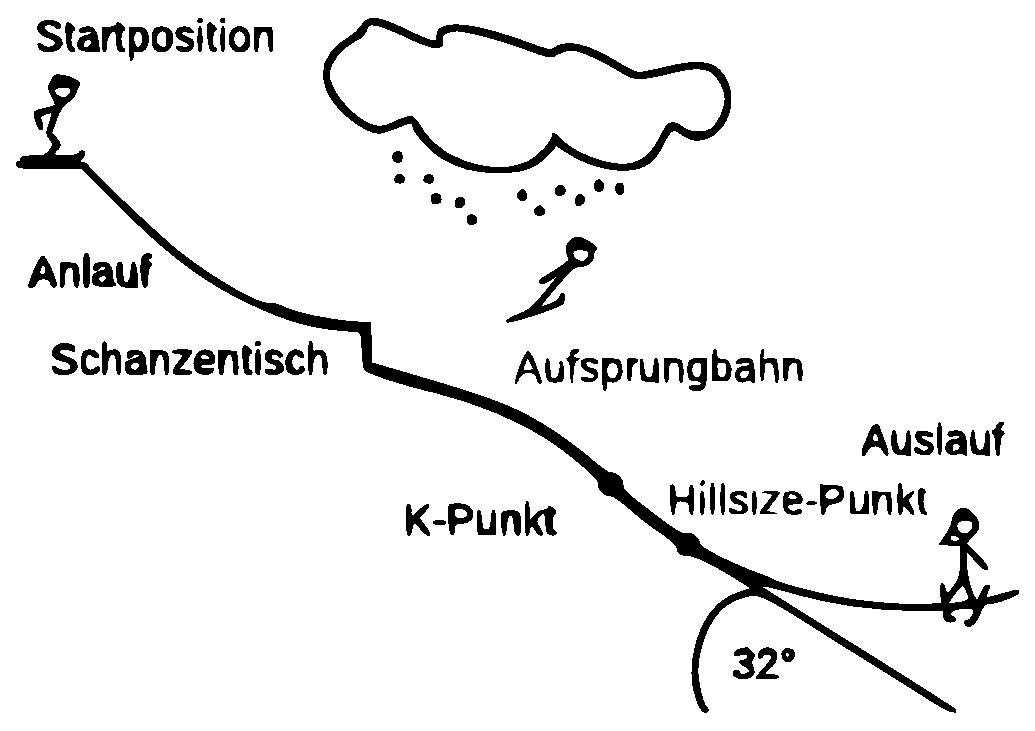
\includegraphics[width=0.5\textwidth]{../_database/Bilder/GrafikAN3331.eps}
\end{center}


In einem Koordinatensystem mit horizontaler x-Achse sei der L�ngsschnitt der Aufsprungbahn der Graph der Funktion $a$. Die steilste Stelle der Aufsprungbahn befindet sich am K-Punkt.
Aufgabenstellung:\leer

Kreuzen Sie die beiden zutreffenden Aussagen an! 

\multiplechoice[5]{  %Anzahl der Antwortmoeglichkeiten, Standard: 5
				L1={Am K-Punkt gilt: $a''(x) < 0$.},   %1. Antwortmoeglichkeit 
				L2={Der K-Punkt ist Wendepunkt der Funktion $a$.},   %2. Antwortmoeglichkeit
				L3={Der K-Punkt ist ein Extrempunkt mit $a'(x) = 0$.},   %3. Antwortmoeglichkeit
				L4={Der K-Punkt ist ein Sattelpunkt. },   %4. Antwortmoeglichkeit
				L5={Am K-Punkt �ndert sich die Kr�mmung des Graphen der Funktion $a$.},	 %5. Antwortmoeglichkeit
				L6={},	 %6. Antwortmoeglichkeit
				L7={},	 %7. Antwortmoeglichkeit
				L8={},	 %8. Antwortmoeglichkeit
				L9={},	 %9. Antwortmoeglichkeit
				%% LOESUNG: %%
				A1=2,  % 1. Antwort
				A2=5,	 % 2. Antwort
				A3=0,  % 3. Antwort
				A4=0,  % 4. Antwort
				A5=0,  % 5. Antwort
				}
				
\end{beispiel}